%\documentclass[english]{beamer}
\documentclass[english,hangout]{beamer}
%\documentclass[aspectratio=169]{beamer}
%\usepackage{amsmath}
%\usepackage{amssymb}
\usepackage{rotating}
\usepackage{verbatim}
\usepackage{latexsym}
\usepackage{graphicx}
\usepackage{tabularx}
\usepackage{ragged2e}
\usepackage{eurosym}   % Euro symbol: \euro
\usepackage{listings}
\usepackage{multirow}
\usepackage{colortbl}
\usepackage{textcomp}  % many special symbols
\usepackage{lmodern}
\usepackage{times}
\usepackage[T1]{fontenc}
\usepackage[utf8]{inputenc}
\usepackage[english]{babel}
\usepackage{booktabs}


\colorlet{punct}{red!60!black}
\definecolor{background}{HTML}{EEEEEE}
\definecolor{delim}{RGB}{20,105,176}
\colorlet{numb}{magenta!60!black}

\lstdefinelanguage{json}{
    basicstyle=\normalfont\ttfamily,
    numbers=left,
    numberstyle=\scriptsize,
    stepnumber=1,
    numbersep=8pt,
    showstringspaces=false,
    breaklines=true,
    frame=lines,
    backgroundcolor=\color{background},
    literate=
     *{0}{{{\color{numb}0}}}{1}
      {1}{{{\color{numb}1}}}{1}
      {2}{{{\color{numb}2}}}{1}
      {3}{{{\color{numb}3}}}{1}
      {4}{{{\color{numb}4}}}{1}
      {5}{{{\color{numb}5}}}{1}
      {6}{{{\color{numb}6}}}{1}
      {7}{{{\color{numb}7}}}{1}
      {8}{{{\color{numb}8}}}{1}
      {9}{{{\color{numb}9}}}{1}
      {:}{{{\color{punct}{:}}}}{1}
      {,}{{{\color{punct}{,}}}}{1}
      {\{}{{{\color{delim}{\{}}}}{1}
      {\}}{{{\color{delim}{\}}}}}{1}
      {[}{{{\color{delim}{[}}}}{1}
      {]}{{{\color{delim}{]}}}}{1},
}

%\usetheme[fb2]{FrankfurtUniversity}
\usetheme[fb2,noslogan]{FrankfurtUniversity}
%\slogan{\large\color{red}UNAUTHORIZED}


\title{Blockchain Solution to \\Healthcare Record System using \\ Hyperledger Fabric}
\subtitle{Final Presentation}
\author{Jathin Sreenivas, Kshitj Yelpale, Varsha Vasudev Kamath}
%\institute{Frankfurt University of Applied Sciences\\}
%\date{\today}
\date{March 31, 2021}

\begin{document}


\begin{frame}
\titlepage
\end{frame}
%\addtocounter{framenumber}{-1}



\begin{frame}
   \frametitle{Agenda}
   \tableofcontents%[hideallsubsections]
\end{frame}



\section{Introduction}




\begin{frame}[fragile]
 \frametitle{Introduction}
 \framesubtitle{Background}
 \begin{itemize}
     \item Specialization in the health care services and patient’s mobility.
     \item Patient’s medical history can help healthcare providers make precise diagnosis and treatment.
     \item Ensuring data integrity, confidentiality and privacy of patients while sharing the clinical data.
 \end{itemize}
\end{frame}



\begin{frame}[fragile]
 \frametitle{Introduction}
 \framesubtitle{Existing Systems}
 \begin{itemize}
     \item Electronic Health Record (EHR) is used to share patient's medical records across different health care providers.
     \item EHR consists of medical information of the patient
in the form of Electronic Medical Record (EMR).
     \item EMR contains a patient’s
medical diagnoses, allergies, history, treatment, and laboratory reports.
     \item Healthcare IT standards are Health Level
7 (HL7), Fast Healthcare Interoperability Resources (FHIR).
\item The other models used by health care providers are push, pull, and view.
 \end{itemize}
\end{frame}



\begin{frame}[fragile]
 \frametitle{Introduction}
 \framesubtitle{Motivation}
    \begin{itemize}
        \item Medical data storing and sharing is an integral part in healthcare systems.
        \item Sharing personal data among various participants through unsecure means can lead to leakage of critical information
        \item  The lack of the a client control over their personal information leads to harmful consequences such as unauthorized identities can access/edit the personal medical details.
        \item  The critical issues in the electronic health/medical records (EHR/EMR) is maintaining the interoperability among various involved identites.
        \item Data security and privacy are also challenges in the current ways of data storing and sharing data through EHR/EMR systems.
    \end{itemize}
\end{frame}

\section{State of the art}


\begin{frame}[fragile]
 \frametitle{State of the art}
 \framesubtitle{What is blockchain?}
    \begin{center}
        \vspace{-1.2em}
            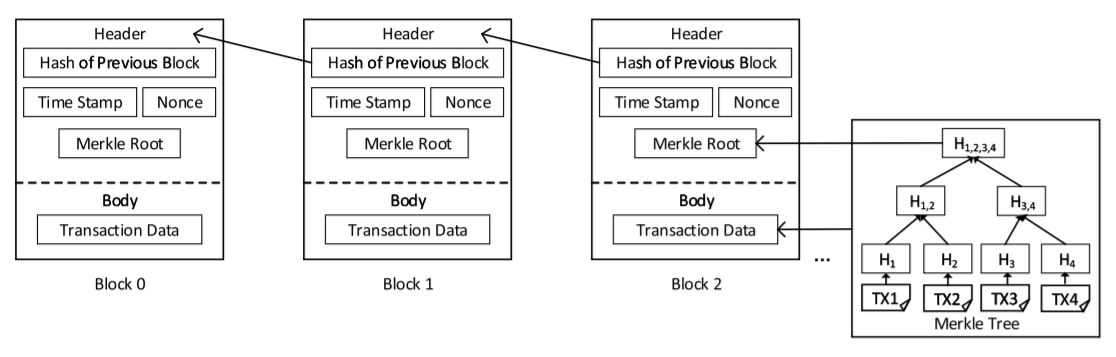
\includegraphics[width=10cm\textwidth,height=5cm]{Block structure.JPG}
            
             \caption{Block Structure \cite{b8}}
        \end{center}
        \vspace{-3mm}
\end{frame}

\begin{frame}[fragile]
 \frametitle{State of the art}
 \framesubtitle{What is blockchain?}
    \begin{center}
        \vspace{-1.2em}
            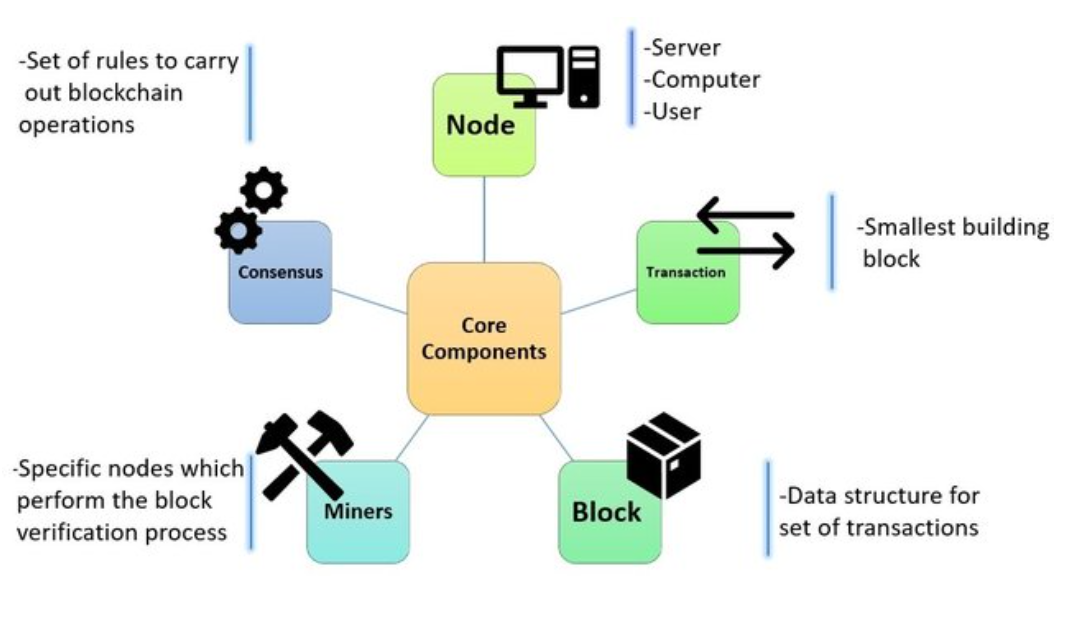
\includegraphics[width=11cm\textwidth,height=5cm]{components.png}
            
             \caption{Blockchain core components \cite{b9}}
        \end{center}
        \vspace{-3mm}
\end{frame}

\begin{frame}[fragile]
 \frametitle{State of the art}
 \framesubtitle{Types of blockchain}
 Public Blockchain (Permissionless)
 \begin{itemize}
     \item Everyone can access the public blockchain and participate in
the transactions.
     \item Fully decentralized.
     \item Examples are Bitcoin, Litecoin, and Ethereum.
 \end{itemize}
 Private Blockchain (Permissioned)
 \begin{itemize}
     \item Restrictions on who can join the
network and who can participate in the transactions.
    \item Used by organizations or companies for its internal usage.
    \item Centralized.
    \item Example, Hyperledger Fabric.
 \end{itemize}
\end{frame}

\section{The Solution}



\begin{frame}[fragile]
 \frametitle{The Solution}
 \framesubtitle{Scenario}
 \begin{itemize}
     \item Map fabric components to EHR systems.
     \item Organizations in fabric mapped to hospitals
     \item Hospitals of same interest connected on same channel. New hospitals will be connected once approved by channel configuration owner hospitals.
     \item Assets in fabric are patient data accessible all over the network.
     \item Store all data in blockchain database
     \item Doctor should see history of a patient to understand condition and prescribe proper medication
     \item Patient should be responsible to make his data available to doctor. 
 \end{itemize}
\end{frame}



\begin{frame}[fragile]
 \frametitle{The Solution}
 \framesubtitle{Why blockchain and fabric?}
    \begin{itemize}
        \item Blockchain stores data cryptographically secure
        \item Authentication and authorization - fabric provides CA and MSP components which provide secure indetities like private key and certificates and validation done when make connection to network.
        \item Confidentiality - fabric is a permisionned blockchain framework.
        \item Availability - distributed nature of blockchain makes data available to all permissioned systems. 
        \item Data integrity - blockchain records are immutable
        \item pBFT consensus algorithm 
        \item Fabric provides history API which helps doctors to analyse a patient's history.
        \item Scalablity - New organization, peers and users with different roles. 
        \item Pluggable modules
    \end{itemize}
\end{frame}



\begin{frame}[fragile]
 \frametitle{The Solution}
 \framesubtitle{Use cases}
    \begin{center}
        \vspace{-1.2em}
            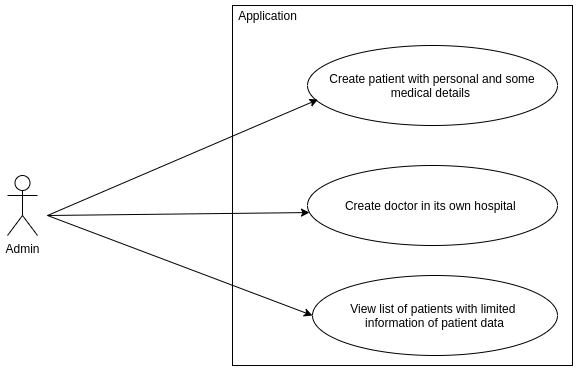
\includegraphics[height=5cm]{Admin use case .png}
        \end{center}
        \vspace{-3mm}
\end{frame}

\begin{frame}[fragile]
 \frametitle{The Solution}
 \framesubtitle{Use cases}
    \begin{center}
        \vspace{-1.2em}
            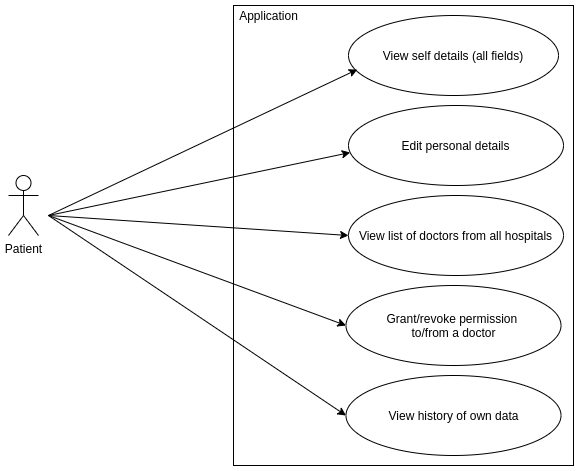
\includegraphics[height=5cm]{Patient use case.png}
        \end{center}
        \vspace{-3mm}
\end{frame}

\begin{frame}[fragile]
 \frametitle{The Solution}
 \framesubtitle{Use cases}
    \begin{center}
        \vspace{-1.2em}
            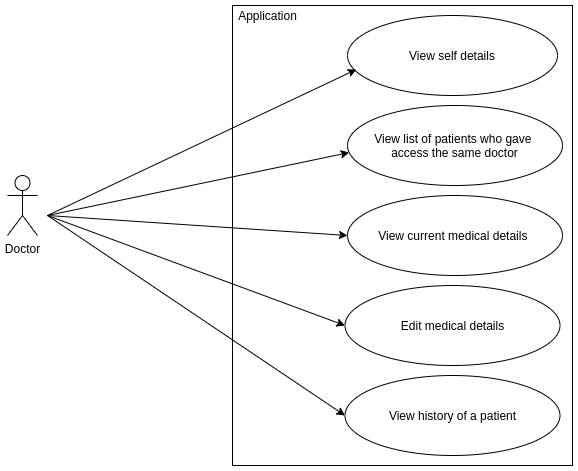
\includegraphics[height=5cm]{Doctor use case.png}
        \end{center}
        \vspace{-3mm}
\end{frame}


\begin{frame}[fragile]
 \frametitle{The Solution}
 \framesubtitle{Architecture}
    \begin{center}
        \vspace{-1.2em}
            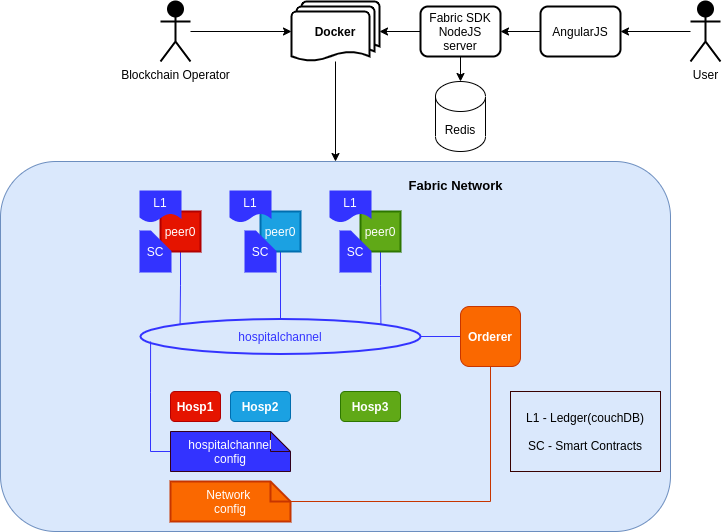
\includegraphics[height=5cm]{Architecture.png}
        \end{center}
        \vspace{-3mm}
\end{frame}



\begin{frame}[fragile]
 \frametitle{The Solution}
 \framesubtitle{Activity diagram - Create Patient}
    \begin{center}
        \vspace{-1.2em}
            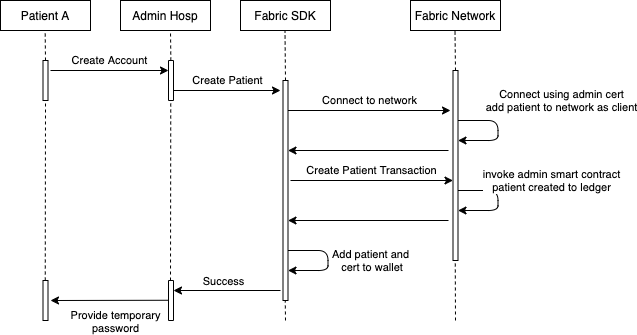
\includegraphics[height=4cm]{firstActivity.png}
        \end{center}
        \vspace{-3mm}
\end{frame}


\begin{frame}[fragile]
 \frametitle{The Solution}
 \framesubtitle{Activity diagram - Create Doctor}
    \begin{center}
        \vspace{-1.2em}
            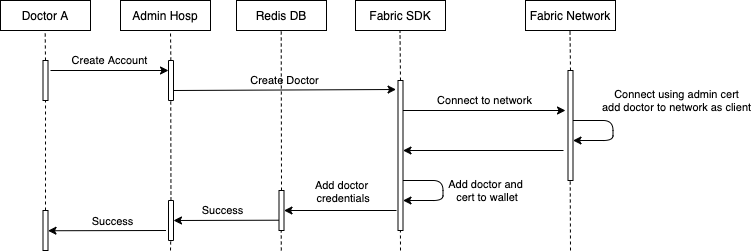
\includegraphics[height=4cm]{secondActivity.png}
        \end{center}
        \vspace{-3mm}
\end{frame}



\begin{frame}[fragile]
 \frametitle{The Solution}
 \framesubtitle{Class diagram - Smart Contract}
    \begin{center}
        \vspace{-1.2em}
            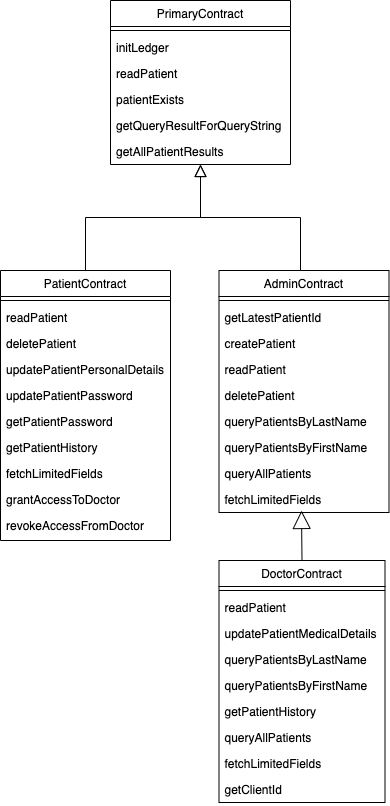
\includegraphics[width=8cm\textwidth, height=6.5cm]{smartContractHierarchy.png}
        \end{center}
        \vspace{-3mm}
\end{frame}
\section{Security Mechanisms}



\begin{frame}[fragile]
 \frametitle{Security Mechanisms}
 \framesubtitle{Private Collections}
    \begin{center}
        \vspace{-1.2em}
            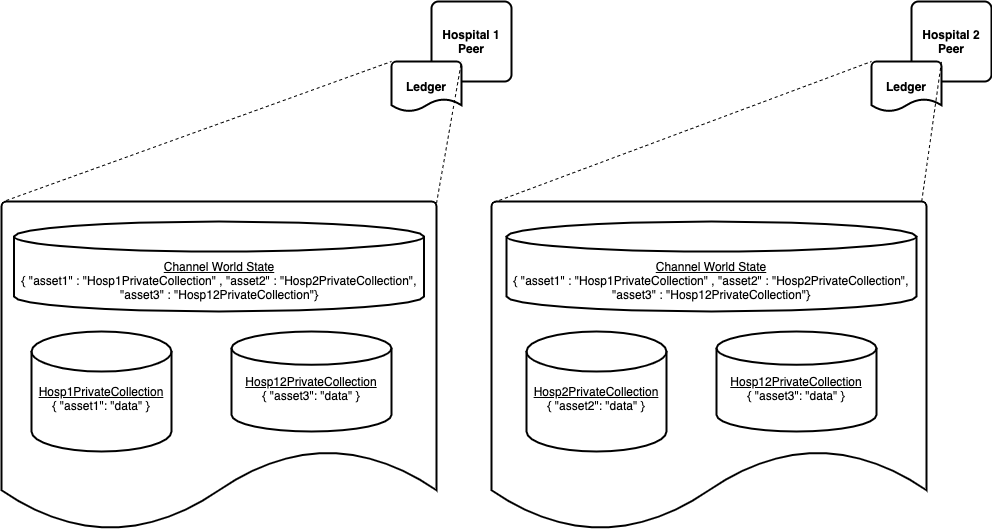
\includegraphics[height=5cm]{PrivateChannel.png}
        \end{center}
        \vspace{-3mm}
\end{frame}



\begin{frame}[fragile]
 \frametitle{Security Mechanisms}
 \framesubtitle{Data re-encryption}
    \begin{center}
        \vspace{-1.2em}
            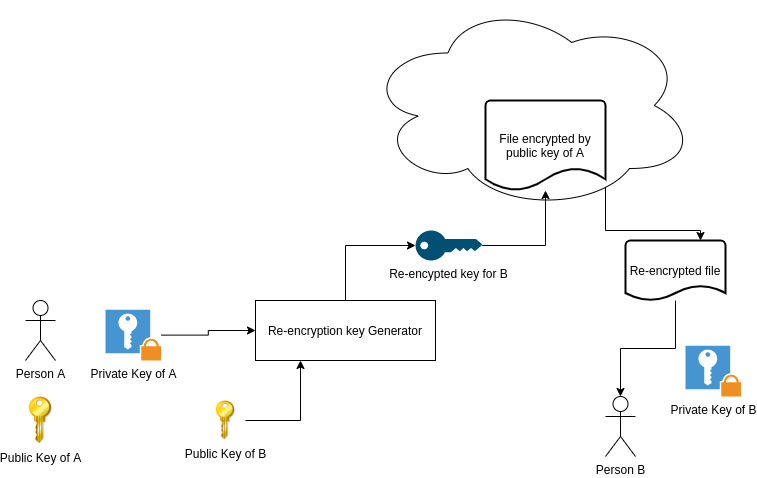
\includegraphics[height=5cm]{Re-encryption.png}
        \end{center}
        \vspace{-3mm}
\end{frame}

\begin{frame}[fragile]
 \frametitle{Security Mechanisms}
 \framesubtitle{Data re-encryption}
    \begin{lstlisting}[language=json,firstnumber=1]
    {
    "patientId": "p1",
    "password": hash(pwd),
    "pwdTemp": true
    "firstName": "abc",
    "lastName" "xyz",
    "data": encrypted patient data using symmetric key,
    "changedBy": "doctorId XX",
    "permissionGranted": [doctorId1: re-encrypted key for doctor 1, doctorId2: re-encrypted key for doctor 2, ...],
    "encryptedSymmetricKey" : "######"
    }    
    \end{lstlisting}
\end{frame}

\section{Demo}


\begin{frame}[fragile]
 \frametitle{Demo}
\end{frame}


\section{Results}



\begin{frame}[fragile]
 \frametitle{Results}
 \framesubtitle{Pros and Cons of using hyperledger Fabric}
 Pros
 \begin{itemize}
     \item Fabric architecture allows to add plugins for the identity management and consensus algorithm.
    \item Confidentiality and security of data can be achieved through MSP.
    \item Performance is optimized, since mining is not required.
    \item Creation of a private channel for only a few participants among
a large blockchain network.
 \end{itemize}
 Cons
 \begin{itemize}
     \item The architecture of hyperledger fabric is quite complex.
     \item It is not a network fault tolerant.
     \item Limited database support.
 \end{itemize}
\end{frame}



\begin{frame}[fragile]
 \frametitle{Results}
 \framesubtitle{Issues in hyperledger}
    \begin{itemize}
        \item getHistoryForKey - Private Data Collection. \cite{b7}
        \item Create a user defined role instead of client. \cite{b6}
        \item Access user attributes using client 
    \end{itemize}
\end{frame}



\begin{frame}[fragile]
 \frametitle{Results}
 \framesubtitle{Challenges in developing application}
    \begin{itemize}
        \item Implementing security mechanism
        \item Re-encryption - Nodejs lacks a decent re-encryption library, need to implement own library
        \item Tracking of public key of created user through fabric SDK
        \item Scaling of peers
    \end{itemize}
\end{frame}

\section{Conclusion}



\begin{frame}[fragile]
 \frametitle{Conclusion}
    \begin{itemize}
        \item Hyperledger fabric is a promissing blockchain framework comes with policies, smart contracts and provision of secure identities. 
        \item Enable the EHR scenario interoperable among multiple hospital organizartions
        \item A promissing framework for private and closed blockchain scenarios
        \item Provide reliable and secure solution in managing medical field records
    \end{itemize}
\end{frame}



\begin{frame}[fragile]
 \frametitle{Conclusion}
 \framesubtitle{Future Work}
    \begin{itemize}
        \item Overcome security challenges
        \item Improve source code to make to provide scalable and pluggable solution in terms of increasing hospitals and peers
        \item Implement powerful ordering service on large scaling of fabric network 
        \item Updation of consortium policies
        \item Wallet can be stored in distributed way with database storage machanism
        \item Bring REST network calls under HTTPS to make data transformation secure using TLS
        \item Integration of email functionality for temporary password of users
        \item Implement functionality of patients
        \item Kubernetes - best tool to deploy and manage production grade application
    \end{itemize}
\end{frame}




\section{References}

\begin{frame}
\frametitle{References}
\begin{thebibliography}{00}

\bibitem{b1} https://www.ncbi.nlm.nih.gov/pmc/articles/PMC7010942/
\bibitem{b2} https://www.ncbi.nlm.nih.gov/pmc/articles/PMC7474412/
\bibitem{b3} https://www.sciencedirect.com/science/article/pii/S2214212-619306155
%\bibitem{b5} https://medium.com/@lichunshen84/build-a-blockchain-poc-application-using-hyperledger-fabric-5a32687072b7, Accessed-On:01/12/2020
\bibitem{b6} https://jira.hyperledger.org/browse/FABC-548, Accessed-On:28/03/2020
\bibitem{b7} https://jira.hyperledger.org/browse/FAB-5094, Accessed-On:28/03/2020
\bibitem{b8} Dynamic Spectrum Management, Signals and Communication by Ying-Chang Liang
\bibitem{b9} https://www.mdpi.com/1099-4300/22/2/175
\bibliography{bibliography}
\end{thebibliography}

\end{frame}


\end{document}